\documentclass[11pt,a4paper]{article}

\usepackage[utf8]{inputenc}
\usepackage[T1]{fontenc}
\usepackage[english]{babel}
\usepackage{lmodern}
\usepackage{microtype}
\usepackage{geometry}
\usepackage{booktabs}
\usepackage{tabularx}
\usepackage{array}
\usepackage{graphicx}
\graphicspath{{figures/}}
\usepackage{hyperref}
\usepackage{enumitem}

\geometry{margin=2.5cm}

\hypersetup{
  colorlinks=true,
  linkcolor=blue,
  citecolor=blue,
  urlcolor=blue
}

\newcolumntype{Y}{>{\raggedright\arraybackslash}X}
\newcommand{\doi}[1]{\href{https://doi.org/#1}{doi:\ #1}}

\title{From Prompt to Process: A Systematic Review of AI-Assisted Software Development Frameworks}
\author{Sanderson Oliveira de Macedo\\
\textit{Federal Institute of Goias}\\
\texttt{sanderson.macedo@ifg.edu.br}}
\date{\today}

\begin{document}

\maketitle

\begin{abstract}
O desenvolvimento de software com IA deixou de ser uma questão de prompts isolados e passou a se organizar em frameworks que estruturam o processo com artefatos persistentes, papéis agênticos, execução integrada e validação. Faltava, porém, uma revisão que tomasse esses frameworks operacionais como objeto, com uma lente de Engenharia de Software, em vez de tratar arquiteturas de agentes de forma abstrata ou técnicas isoladas do ciclo de vida. Este artigo apresenta uma revisão sistemática de literatura conduzida sob o protocolo de Kitchenham, que reuniu 37 estudos publicados entre 2022 e 2026 após triagem em duas passadas e três rodadas de snowballing, incluindo apenas artigos acadêmicos e preprints arquivados com registro verificável. A síntese temática em modo híbrido derivou seis temas indutivos e os confrontou com uma taxonomia proposta de seis dimensões (especificação, contexto, papéis, execução, validação e portabilidade). Os resultados sustentam empiricamente o deslocamento do prompt para o processo, presente em 34 dos 37 estudos, e validam cinco das seis dimensões; portabilidade é fraca e quase sempre diagnóstica, e dois eixos emergem fora da taxonomia, a colaboração humano-IA e a segurança. Identificamos três eixos de tensão recorrentes e mostramos que contexto e rastreabilidade, e não a geração de código em si, são os gargalos práticos transversais. Concluímos com uma agenda de pesquisa orientada a processo, centrada em benchmarks que avaliem o pipeline, comparação direta entre frameworks e avaliação longitudinal de governança.
\end{abstract}

\noindent\textbf{Palavras-chave:} desenvolvimento de software com IA; agentes de IA; revisão sistemática; engenharia de software; frameworks agênticos.

\section{Introdução}

A programação assistida por modelos de linguagem mudou de natureza em poucos anos. O que começou como sugestão de trechos de código a partir de prompts isolados evoluiu para sistemas que decompõem o ciclo de desenvolvimento entre agentes especializados, mantêm artefatos persistentes, executam ferramentas e validam o próprio trabalho. ChatDev e MetaGPT mostraram que organizar agentes por papéis de engenharia, e não apenas melhorar o prompt, muda o que o sistema consegue entregar \cite{ChenQian2023,SiruiHong2023}. A literatura mais recente já fala em uma Engenharia de Software nativa de IA e trata sistemas multiagente como linha de pesquisa própria \cite{hou2024llmse,AhmedEHassan2024,JundaHe2025}. A unidade de trabalho, antes o prompt, tornou-se o processo.

Esse deslocamento traz um objeto novo: o framework operacional que organiza o desenvolvimento sobre um agente. Caracterizá-lo exige examinar a função de cada mecanismo, como a especificação dirige a geração, como o contexto do repositório é recuperado, como papéis são distribuídos, como a execução age sobre o ambiente e como a validação ancora o resultado, em vez de métricas superficiais como número de comandos ou popularidade. As revisões existentes, porém, abordam o problema por outro ângulo. Parte da literatura classifica arquiteturas de agentes de forma abstrata, por componentes cognitivos, e parte mapeia técnicas de modelos de linguagem por tarefas isoladas do ciclo de vida. Falta uma lente de Engenharia de Software voltada para os frameworks que organizam o ciclo de desenvolvimento em nível de processo e de repositório, e falta confrontar a estrutura desses frameworks com a evidência disponível, em vez de descrevê-los um a um.

Para preencher essa lacuna, conduzimos uma revisão sistemática de literatura sob o protocolo de Kitchenham, restrita a artigos acadêmicos e preprints arquivados com registro verificável \cite{kitchenham2009slr}. A partir de um corpus final de 41 estudos publicados entre 2022 e 2026, propomos uma taxonomia de seis dimensões para classificar esses frameworks e a confrontamos com a evidência do corpus, por meio de uma síntese temática em modo híbrido. As contribuições deste artigo são três: uma taxonomia de seis dimensões (especificação, contexto, papéis, execução, validação e portabilidade) testada contra a evidência, e não assumida a priori; uma síntese temática de seis temas indutivos que cobre 100\% do corpus e expõe três eixos de tensão e dois eixos emergentes fora da taxonomia; e uma agenda de pesquisa orientada a processo que decorre diretamente das lacunas observadas.

A revisão é guiada por cinco perguntas de pesquisa. RQ1: quais dimensões arquiteturais distinguem esses frameworks? RQ2: como eles organizam contexto, papéis, artefatos, execução e validação? RQ3: que tipos de evidência sustentam as alegações? RQ4: quais riscos e limitações são reportados ou inferíveis? RQ5: que lacunas de pesquisa permanecem para comparar, avaliar e governar esses frameworks em projetos reais? O restante do artigo está organizado da seguinte forma: o Método de Revisão descreve o protocolo e o fluxo de seleção; os Trabalhos Relacionados posicionam a revisão frente à literatura existente; a Taxonomia Proposta apresenta as seis dimensões; os Resultados e Síntese consolidam os seis temas e confrontam a taxonomia com a evidência; a Discussão expõe os achados transversais e os eixos de tensão; e a Agenda de Pesquisa e a Conclusão delineiam os próximos passos.

\section{Método de Revisão}

A Introdução situou os frameworks de apoio ao desenvolvimento de software com IA como uma camada que organiza o trabalho de quem usa um agente de desenvolvimento, e argumentou que compará-los exige examinar a função de cada mecanismo, e não métricas superficiais como número de comandos ou popularidade. Investigar esse objeto impõe uma restrição metodológica: os frameworks mais relevantes circulam fora de venues acadêmicos, em repositórios abertos, documentação oficial e kits comunitários, de modo que uma revisão restrita a artigos indexados deixaria de cobri-los. Por isso, esta revisão foi conduzida como uma revisão de literatura multivocal (Multivocal Literature Review, MLR), que combina, sob um único protocolo, o rigor da revisão sistemática de Kitchenham para a literatura formal e as diretrizes de Garousi, Felderer e Mäntylä para a literatura cinzenta \cite{kitchenham2009slr,garousi2019mlr}. A data de corte foi 26 de maio de 2026 e a janela de cobertura, de 2018 a 2026.

Os dois corpora cumprem papéis distintos e complementares. A literatura formal, composta por artigos e preprints recuperados em bases acadêmicas, fundamenta as dimensões de análise da taxonomia e estabelece o estado do conhecimento sobre agentes, especificação, validação e riscos. A literatura cinzenta, composta pelas fontes primárias dos frameworks de apoio, fornece os objetos efetivamente caracterizados por essas dimensões. O protocolo foi fixado antes da execução e define as perguntas de pesquisa, as fontes consultadas, os critérios de inclusão e exclusão, o esquema de extração e a estratégia de snowballing. A Figura~\ref{fig:metodologia} resume o fluxo de levantamento da literatura formal, da identificação ao relato, com as contagens reais de cada etapa.

\begin{figure}[h!]
\centering
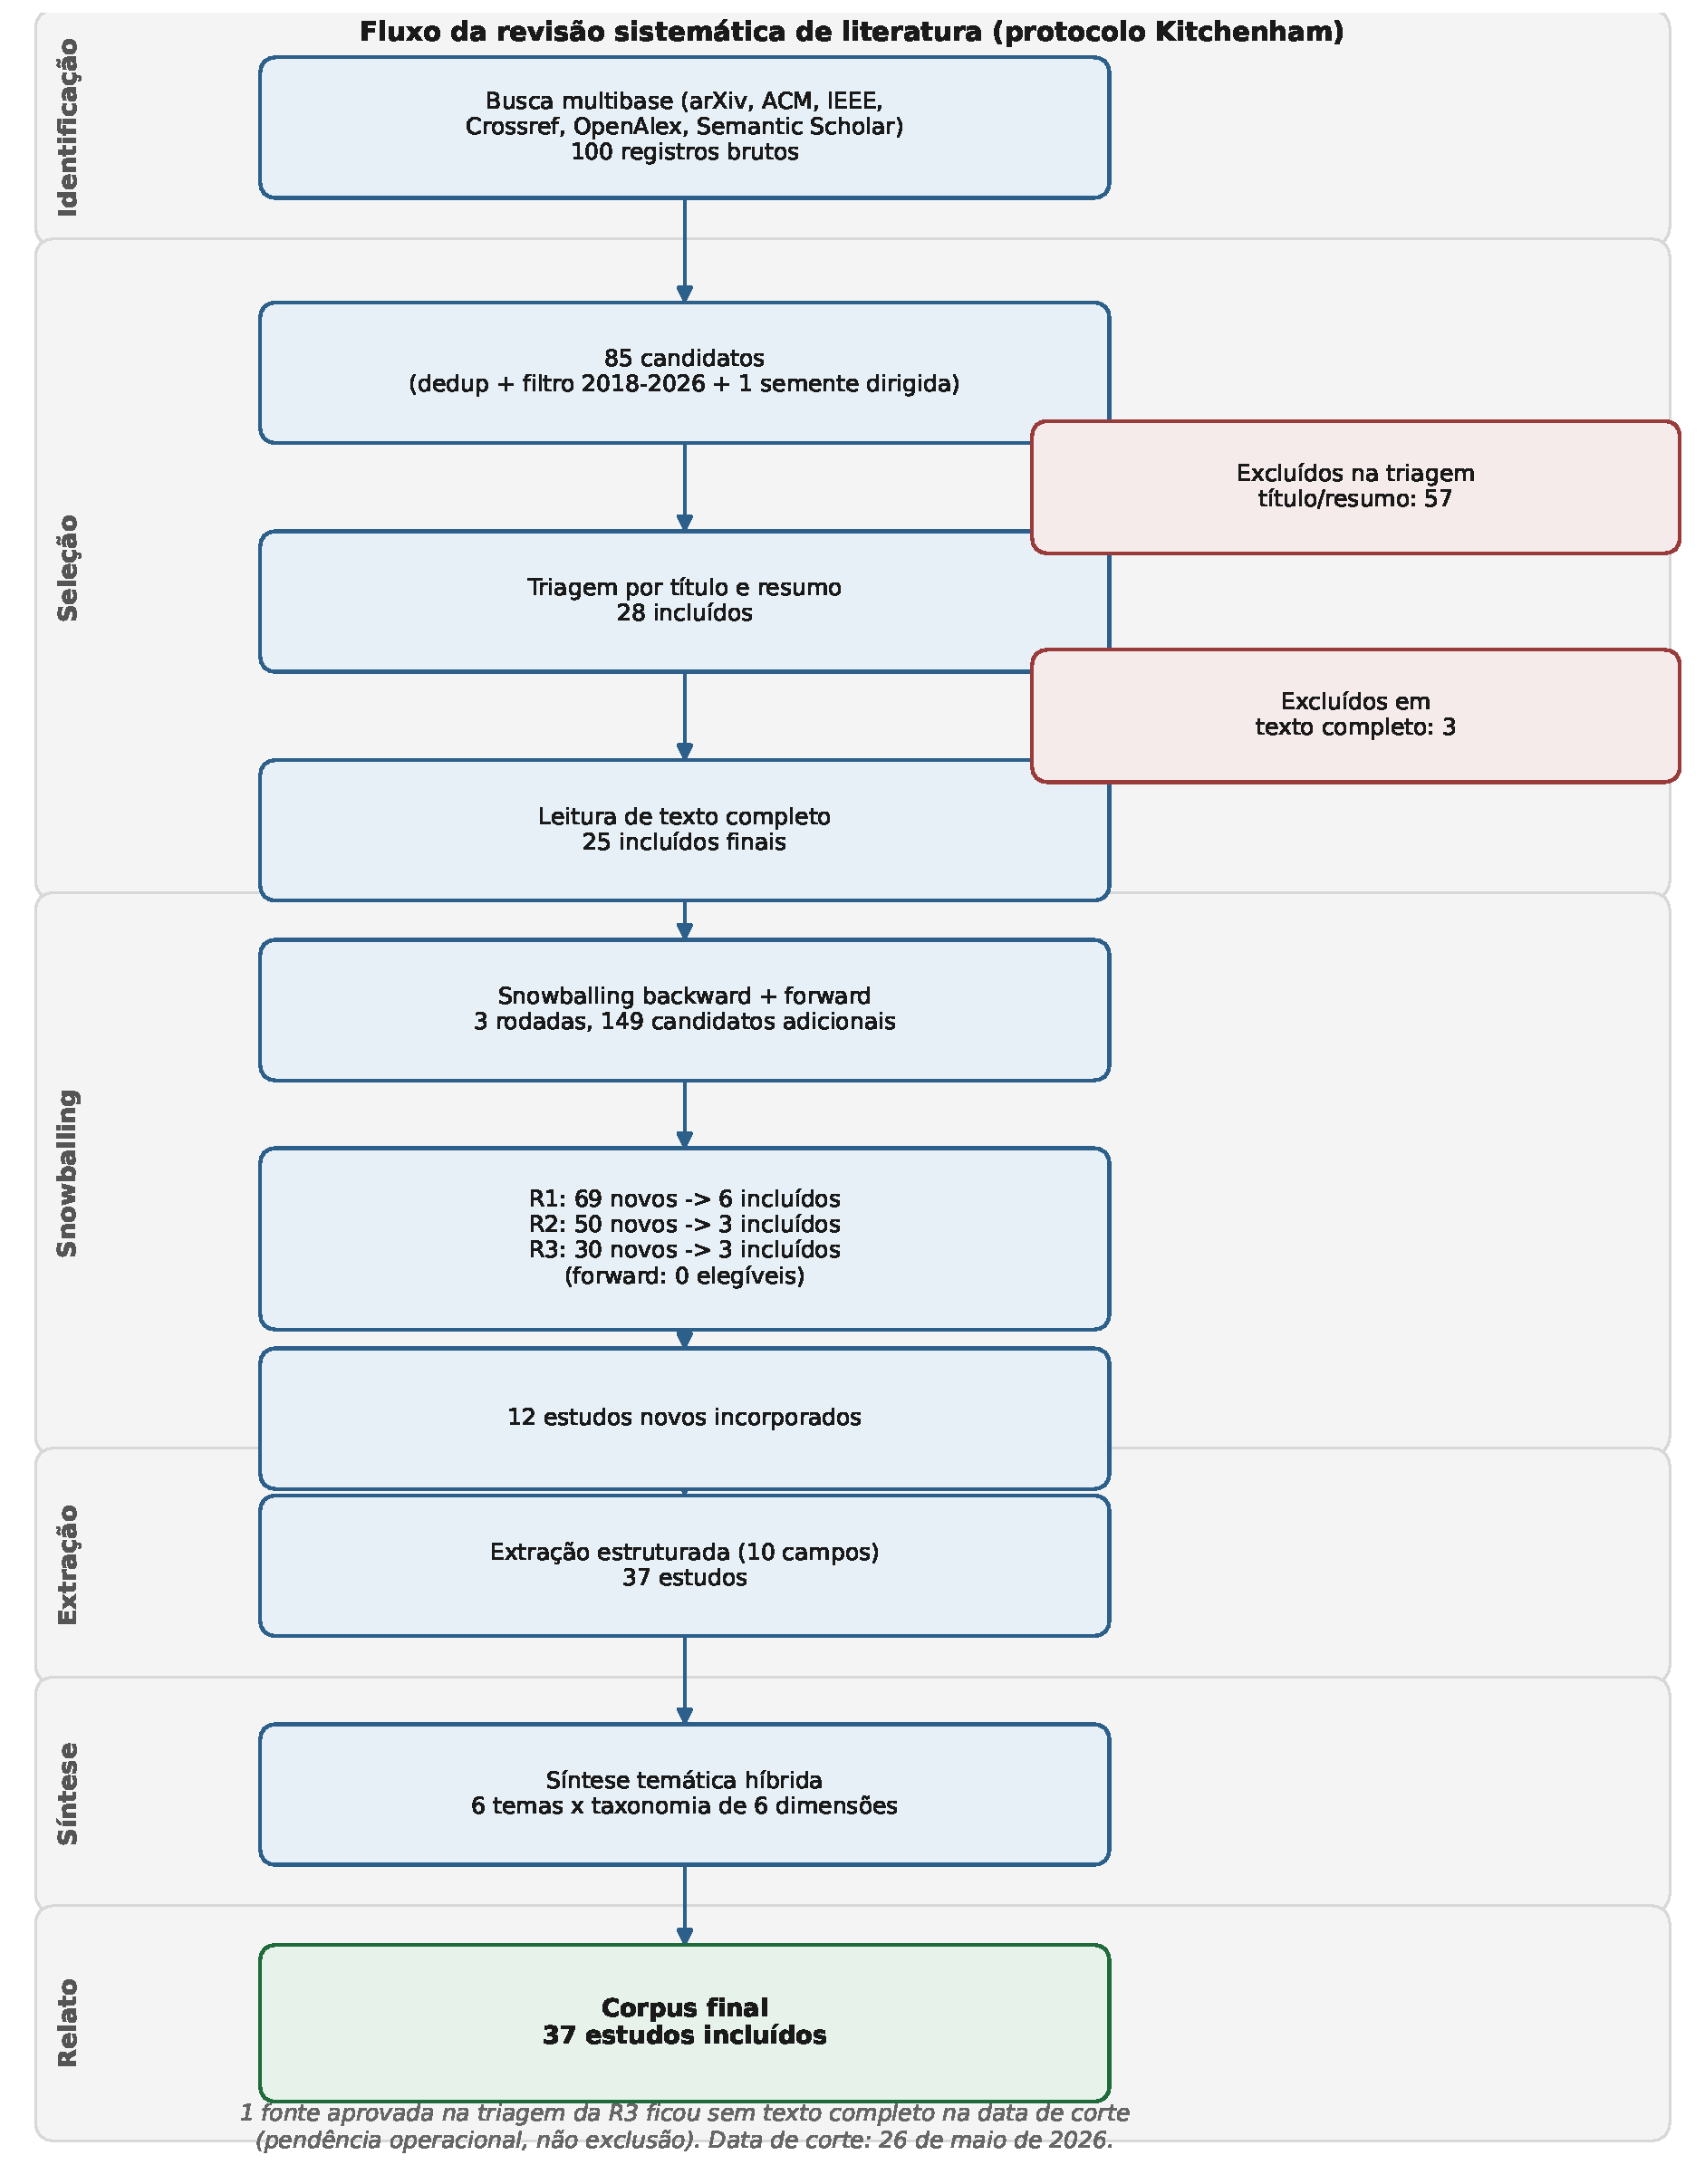
\includegraphics[width=0.92\textwidth]{methodology_pt.pdf}
\caption{Fluxo da revisão de literatura multivocal aplicado à literatura formal, do protocolo Kitchenham ao relato, com as contagens reais de cada etapa.}
\label{fig:metodologia}
\end{figure}

A revisão é orientada pelas cinco perguntas de pesquisa apresentadas na Introdução (RQ1 a RQ5); a RQ5, sobre as lacunas que permanecem para comparar, avaliar e governar esses frameworks em projetos reais, é uma questão de nível de síntese, respondida transversalmente na Agenda de Pesquisa, e por isso a matriz de extração registra apenas RQ1 a RQ4 por estudo.

A busca seguiu duas estratégias. Para a literatura formal, consultaram-se de forma automatizada arXiv, ACM Digital Library, IEEE Xplore, Crossref, OpenAlex e Semantic Scholar, com Scopus e Web of Science acessados por metadados abertos via OpenAlex e o Google Scholar usado para verificação de citações. Os descritores foram organizados em quatro blocos conceituais (desenvolvimento assistido por IA, engenharia de software agêntica, especificação como artefato e organização por workflows), com strings booleanas adaptadas a cada base e documentadas no protocolo. Para a literatura cinzenta, em que a busca por string não se aplica, adotou-se busca dirigida às fontes primárias dos frameworks (documentação oficial, repositórios e blogs de produto), com critérios próprios de escopo e tração detalhados adiante; o esquema de extração, porém, foi o mesmo nas duas vertentes.

Os critérios de elegibilidade da literatura formal foram fixados no protocolo e estão resumidos na Tabela~\ref{tab:criterios}. A regra de decisão é agregada: uma fonte que não satisfaz o critério I1 é excluída; entre as fontes que satisfazem I1, são incluídas apenas as que satisfazem ao menos dois dos critérios I2, I3 e I4. Os motivos de exclusão foram registrados de forma operacional para cada fonte descartada, permitindo o relato auditável das razões de descarte em cada passada.

\begin{table}[h!]
\centering
\caption{Critérios de inclusão e exclusão aplicados na seleção dos estudos.}
\label{tab:criterios}
\small
\begin{tabularx}{\textwidth}{@{}p{0.46\textwidth}Y@{}}
\toprule
\textbf{Critérios de inclusão} & \textbf{Critérios de exclusão} \\
\midrule
I1: descreve framework, método, toolkit, plataforma, IDE, CLI ou kit que organiza o desenvolvimento com IA em mais de uma etapa. & E1: trata apenas de modelos de linguagem, APIs ou benchmarks de código, sem camada de processo. \\
I2: descreve produção ou consumo de artefatos persistentes (specs, planos, PRDs, tarefas, logs, evidências). & E2: descreve assistente de código genérico, sem artefatos persistentes, papéis, comandos ou validação própria. \\
I3: define papéis, agentes, personas, skills, workflows ou comandos de coordenação. & E3: discute LLMs para uma única tarefa isolada, sem proposta de framework ou processo. \\
I4: descreve integração com execução de código, testes, terminal, IDE, navegador ou repositórios. & E4: é puramente promocional, sem critérios, arquitetura ou evidência rastreável. \\
I5: fonte acadêmica, oficial ou comunitária tecnicamente verificável. & E5: é duplicata de outra fonte mais completa ou mais recente. \\
I6: disponível em inglês ou português. & E6: está abandonada ou inacessível para verificação. \\
I7: publicada ou atualizada entre 2018 e 2026. & E7: é apenas resumo, slide, anúncio breve ou opinião sem detalhe técnico. \\
I8: permite extrair pelo menos quatro campos do esquema de extração. & E8: menciona os frameworks apenas tangencialmente, sem análise substantiva. \\
\bottomrule
\end{tabularx}
\end{table}

Na literatura formal, a busca multibase retornou 100 registros brutos, reduzidos a 85 candidatos após a deduplicação por DOI e título, a aplicação do filtro temporal de 2018 a 2026 e a inclusão de uma semente dirigida pertencente ao escopo inicial e ausente da recuperação automática. Esses 85 candidatos passaram por uma primeira triagem de título e resumo, que incluiu 28 estudos para leitura de texto completo e excluiu 57. Na segunda passada, os 28 textos completos foram lidos integralmente sob os mesmos critérios, resultando em 25 estudos incluídos e 3 excluídos. As contagens e os motivos de exclusão de ambas as passadas foram registrados em log append-only para auditoria.

A partir dos 25 estudos incluídos, aplicou-se snowballing backward e forward segundo as diretrizes de Wohlin \cite{wohlin2014snowballing}, com um nível de profundidade e limite de três rodadas, cada uma semeada pelos incluídos da anterior. As três rodadas geraram, respectivamente, 69, 50 e 30 candidatos novos; destes, 9, 5 e 4 avançaram para texto completo e 6, 3 e 3 foram incluídos, e a busca forward não retornou citações elegíveis em nenhuma rodada. Ao todo, foram examinados 149 candidatos adicionais e incorporados 12 estudos novos, consolidando o corpus final em 37 estudos incluídos. Uma fonte aprovada na triagem da terceira rodada ficou sem texto completo na data de corte e foi mantida como pendência operacional, não como exclusão.

A revisão foi conduzida como multivocal por uma razão de cobertura: parte expressiva dos frameworks que organizam o desenvolvimento sobre um agente circula em fontes primárias não indexadas, como documentação oficial, repositórios e blogs de produto, de modo que restringir a revisão a artigos indexados deixaria essa camada de fora. A vertente de literatura cinzenta foi, portanto, levantada por busca dirigida a essas fontes primárias, sob o mesmo esquema de extração da literatura formal, mas com critérios próprios de escopo e tração. A caracterização aprofundada dos frameworks de apoio ao desenvolvimento por quem utiliza um agente, como GitHub Spec Kit, OpenSpec, BMAD Method, Get Shit Done e Spec Kitty, é reportada em um estudo companheiro dedicado a esse recorte; este artigo concentra-se no corpus formal de 37 estudos, que estabelece a estrutura e as tensões do campo. Reversa integra esse corpus formal por ter entrado como semente dirigida na busca.

De cada estudo incluído foram extraídos dez campos estruturados: nome, natureza, origem, artefatos, papéis, execução, validação, portabilidade, evidência e riscos. A consolidação da extração em matriz permitiu comparar os estudos de forma uniforme. A síntese seguiu abordagem temática em modo híbrido: temas indutivos foram identificados a partir das fichas de extração e, em seguida, confrontados com a taxonomia de seis dimensões proposta na revisão (especificação, contexto, papéis, execução, validação e portabilidade), reportando a sobreposição, as dimensões pouco cobertas e os temas que emergem fora da taxonomia.

Por fim, registre-se que a avaliação formal de qualidade por checklist não foi aplicada nesta rodada: a força da evidência é classificada por categoria de fonte, distinguindo estudo empírico, paper conceitual, documentação oficial e repositório público. Como repositórios e documentação de ferramentas mudam rapidamente, observações sobre versões, integrações, releases ou comandos devem ser lidas como um retrato do corpus consultado na data de corte, não como propriedades estáveis dos frameworks. As demais limitações que delimitam a leitura dos resultados são consolidadas na seção de Limitações da Revisão.

\section{Trabalhos Relacionados}

A literatura que antecede esta revisão organiza-se em duas vertentes, e o posicionamento deste estudo decorre da lacuna entre elas.

\noindent\textbf{Revisões de agentes e de Engenharia de Software com IA.} A primeira vertente reúne revisões e visões que mapeiam o uso de modelos de linguagem e de agentes na Engenharia de Software. Hou et al. conduzem uma revisão sistemática ampla do uso de modelos de linguagem em tarefas de Engenharia de Software, organizada por etapa do ciclo de vida e por técnica \cite{hou2024llmse}; He, Treude e Lo revisam a arquitetura interna e a cooperação de sistemas multiagente baseados em modelos de linguagem, delineando um roteiro para a consolidação desses sistemas \cite{JundaHe2025}; e Hassan et al. propõem a visão de uma Engenharia de Software nativa de IA, com um roteiro de desafios para o que chamam de Engenharia de Software 3.0 \cite{AhmedEHassan2024}. Essas contribuições são valiosas para entender a anatomia dos agentes e a direção do campo. Mas operam em um nível de abstração que classifica modelos, componentes cognitivos e técnicas por tarefa, ou que projeta cenários futuros. Nenhuma caracteriza os frameworks operacionais que, no presente, organizam o trabalho de desenvolvimento sobre um agente em nível de processo e de repositório.

\noindent\textbf{Propostas orientadas a processo.} A segunda vertente é formada pelos próprios frameworks que estruturam o processo. O desenvolvimento orientado por especificação articula a especificação como contrato vivo na era dos assistentes de codificação \cite{DeepakBabuPiskala2026}; a distinção entre codificar por intuição e codificar de forma agêntica formaliza um espectro de autonomia com implicações práticas \cite{RanjanSapkota2025}; e frameworks como MetaGPT, ChatDev e Reversa instanciam, cada um a seu modo, a organização do ciclo por papéis, artefatos e validação \cite{SiruiHong2023,ChenQian2023,Macedo2026}. Cada uma dessas propostas, porém, avalia a si mesma de forma isolada, sem um referencial comum que permita compará-las.

\noindent\textbf{Posicionamento.} Entre uma literatura de revisão que descreve agentes de forma abstrata e uma literatura de propostas que avalia cada framework isoladamente, falta uma revisão sistemática que tome os frameworks operacionais como objeto, com uma lente de Engenharia de Software, e que confronte a estrutura desses frameworks com a evidência disponível por meio de um referencial explícito. É essa a contribuição deste artigo: uma taxonomia de seis dimensões confrontada com a evidência de um corpus de 41 estudos, uma síntese temática que expõe os eixos de tensão do campo e uma agenda de pesquisa orientada a processo. O diferencial é mensurável pela unidade de análise: enquanto Hou et al. organizam o uso de modelos de linguagem por atividade do ciclo de vida e por técnica \cite{hou2024llmse}, e He et al. organizam os sistemas multiagente por componente arquitetural e de cooperação \cite{JundaHe2025}, esta revisão toma o framework operacional como unidade e classifica os 41 estudos por seis dimensões de processo, com seis temas indutivos que cobrem 100\% do corpus. Onde aquelas revisões respondem o que modelos e agentes fazem por tarefa, esta responde como o processo de desenvolvimento é estruturado sobre o agente. Diferente das comparações de produto voltadas a praticantes, o foco aqui é o corpus de literatura e a estrutura que dele emerge, não a recomendação de uma ferramenta específica.

\section{Taxonomia Proposta}

Para classificar os frameworks do corpus de forma uniforme, propomos uma taxonomia de seis dimensões: especificação, contexto, papéis, execução, validação e portabilidade. Essas dimensões foram escolhidas por aparecerem repetidamente, ainda que com nomes diferentes, nos estudos analisados, e correspondem aos campos estruturados extraídos de cada estudo. A taxonomia é apresentada aqui como referencial; sua validação empírica contra o corpus, incluindo as dimensões fortes e as fracas, é reportada na seção de Resultados. A Tabela~\ref{tab:taxonomia} resume cada dimensão por uma pergunta orientadora e por indicadores observáveis.

\noindent\textbf{Especificação.} Descreve como o framework transforma intenções humanas em artefatos que orientam o trabalho do agente. No extremo mais fraco, a especificação é apenas um prompt; no mais forte, é um conjunto versionado de requisitos, critérios de aceitação, planos, tarefas, arquitetura e políticas. O desenvolvimento orientado por especificação torna essa dimensão explícita ao tratar a especificação como contrato versionável que dirige a geração \cite{DeepakBabuPiskala2026}, e AgileGen a operacionaliza por meio de critérios de aceitação executáveis \cite{SaiZhang2025}. Reversa desloca a origem da especificação: em vez de partir de um produto novo, recupera especificações operacionais a partir de sistemas existentes \cite{Macedo2026}.

\noindent\textbf{Contexto.} É o mecanismo pelo qual o framework decide o que o agente deve saber antes de agir, o que inclui documentos, código, histórico, decisões arquiteturais, regras locais e evidências coletadas. A engenharia de contexto é tratada como disciplina própria para agentes que operam sobre repositórios reais \cite{SeyedmoeinMohsenimofidi2025}, e AutoCodeRover demonstra que a recuperação estrutural do contexto no código melhora a qualidade das correções geradas \cite{YuntongZhang2024}. Em Reversa, o contexto é extraído do legado e rotulado por confiança \cite{Macedo2026}.

\noindent\textbf{Papéis.} Definem especialização, autoridade e expectativa de comportamento. Frameworks multiagente distribuem tarefas entre personas como gerente de produto, arquiteto, desenvolvedor, testador e revisor, o que reduz a ambiguidade do prompt e cria expectativas de saída. MetaGPT é o caso mais explícito, ao internalizar procedimentos operacionais padrão e atribuir artefatos específicos a cada papel \cite{SiruiHong2023}, enquanto ChatDev e CodePori mostram que a decomposição por papéis já era uma linha ativa de pesquisa \cite{ChenQian2023,ZeeshanRasheed2024}.

\noindent\textbf{Execução.} Indica se o framework apenas produz orientação ou se também aciona ferramentas, edita código, roda testes e interage com interfaces. Ferramentas agênticas modernas tornam a execução uma dimensão central: o agente não apenas recomenda, mas modifica o ambiente. AutoDev e AutoCodeRover operam diretamente sobre o repositório, editando código e executando testes em tarefas reais de melhoria de programas \cite{MicheleTufano2024,YuntongZhang2024}, e Prompt Sapper materializa a execução como uma plataforma de produção de cadeias de IA \cite{YuCheng2023}.

\noindent\textbf{Validação.} Compreende os mecanismos para verificar se o que foi produzido está correto, completo e alinhado ao contexto, o que pode incluir testes automatizados, revisão humana, artefatos de evidência, traços auditáveis e gates de prontidão. O asseguramento baseado em traços articula contratos, testes e governança \cite{Paduraru2026}; a colaboração verificável entre assistentes torna auditável cada ato do fluxo \cite{Merchant2025}; e Reversa explicita confiança e lacunas nos artefatos recuperados \cite{Macedo2026}. A validação é crítica porque agentes podem produzir resultados plausíveis sem aderência real ao sistema.

\noindent\textbf{Portabilidade.} Descreve se o framework depende de um fornecedor, IDE, modelo ou formato específico. No corpus, esta é a dimensão mais frágil: ela aparece quase sempre pelo lado negativo, como risco de aprisionamento e de dependência de plataforma, e o aprisionamento só é nomeado explicitamente em um estudo \cite{SeyedmoeinMohsenimofidi2025}. Quase nenhum framework trata portabilidade como propriedade de projeto positiva e deliberada, o que justifica lê-la como dimensão predominantemente diagnóstica, conforme detalhado na seção de Resultados.

\begin{table}[h!]
\centering
\caption{Dimensões da taxonomia proposta.}
\label{tab:taxonomia}
\small
\begin{tabularx}{\textwidth}{p{2.8cm}Y Y}
\toprule
\textbf{Dimensão} & \textbf{Pergunta orientadora} & \textbf{Indicadores observáveis} \\
\midrule
Especificação & Como a intenção vira contrato de trabalho? & Specs, PRDs, planos, stories, tarefas, critérios de aceitação \\
Contexto & Como o agente sabe o que é relevante? & Repositório, docs, hooks, regras, memória, evidências, lacunas \\
Papéis & Quem decide, quem implementa e quem revisa? & Personas, agentes, skills, responsabilidades, autoridade \\
Execução & O framework age no ambiente ou apenas orienta? & Edição de código, comandos, testes, navegador, terminal, IDE \\
Validação & Como erros são detectados antes de virarem entrega? & Testes, checklists, gates, artefatos, revisão humana, confiança \\
Portabilidade & O processo sobrevive fora de uma ferramenta? & Múltiplas integrações, formatos abertos, aprisionamento, instalação local \\
\bottomrule
\end{tabularx}
\end{table}

\section{Resultados e Síntese}

Esta seção consolida os achados dos 37 estudos incluídos. A síntese segue uma abordagem temática em modo híbrido: seis temas foram derivados indutivamente dos campos estruturados das fichas de extração (artefatos, papéis, execução, validação, portabilidade, riscos, natureza e evidência) e, em seguida, confrontados com a taxonomia de seis dimensões proposta na seção anterior, de modo a testá-la contra a evidência em vez de assumi-la. Os temas respondem às perguntas RQ1 a RQ4; a RQ5, sobre lacunas, é tratada na Agenda de Pesquisa. A força da evidência de cada estudo é ponderada por uma avaliação de qualidade por categoria de fonte, descrita no Método e resumida adiante (Tabela~\ref{tab:qualidade}).

\noindent\textbf{Panorama quantitativo.} A Tabela~\ref{tab:quant} resume a composição do corpus. A categoria framework domina quase por completo (34 dos 37 estudos), o que sustenta empiricamente a tese de que a unidade de trabalho se deslocou do prompt isolado para o processo estruturado. A avaliação empírica é reivindicada por 26 estudos e 22 disponibilizam repositório público, mas dez são preprints arXiv ainda não revisados por pares, o que exige leitura qualificada da força da evidência (Figura~\ref{fig:evidence}). A distribuição temporal mostra aceleração consistente do campo, de um único estudo em 2022 para onze em 2026, com a maior parte do corpus concentrada a partir de 2024 (Figura~\ref{fig:year}). Os venues são dispersos, com a ACM Transactions on Software Engineering and Methodology como canal recorrente (cinco estudos) seguido de uma cauda longa de conferências e periódicos com um a dois estudos cada, o que é coerente com um campo emergente ainda sem foro consolidado.

\begin{table}[h!]
\centering
\caption{Composição do corpus de 37 estudos incluídos. Contagens extraídas da matriz de extração.}
\label{tab:quant}
\small
\begin{tabularx}{\textwidth}{@{}p{0.50\textwidth}r Y@{}}
\toprule
\textbf{Aspecto} & \textbf{N} & \textbf{Observação} \\
\midrule
Total de estudos incluídos & 37 & Após triagem em duas passadas e três rodadas de snowballing \\
Natureza: framework & 34 & Predominância quase total \\
Natureza: arquitetura / plataforma / método & 1 / 1 / 1 & JulesWhite2023, YuCheng2023, JSauvola2024 \\
Com avaliação empírica & 26 & Algum grau de validação reivindicado \\
Com repositório público & 22 & Rastreabilidade de código em mais da metade \\
Preprint arXiv & 10 & Literatura ainda não revisada por pares \\
Survey ou revisão & 2 & AhmedEHassan2024, JundaHe2025 \\
Estudo de caso & 5 & Ulfsnes2024, ZeeshanRasheed2024, Baron2025, Khan2026, Macedo2026 \\
Distribuição por ano & \multicolumn{2}{l}{2022:1, 2023:4, 2024:10, 2025:11, 2026:11} \\
Origem acadêmica ou técnica / industrial & 33 / 4 & Quatro estudos de indústria ou prática profissional \\
Confiança de extração alta & 35 & Média em Dam2025 e JundaHe2025 \\
\bottomrule
\end{tabularx}
\end{table}

\begin{figure}[h!]
\centering
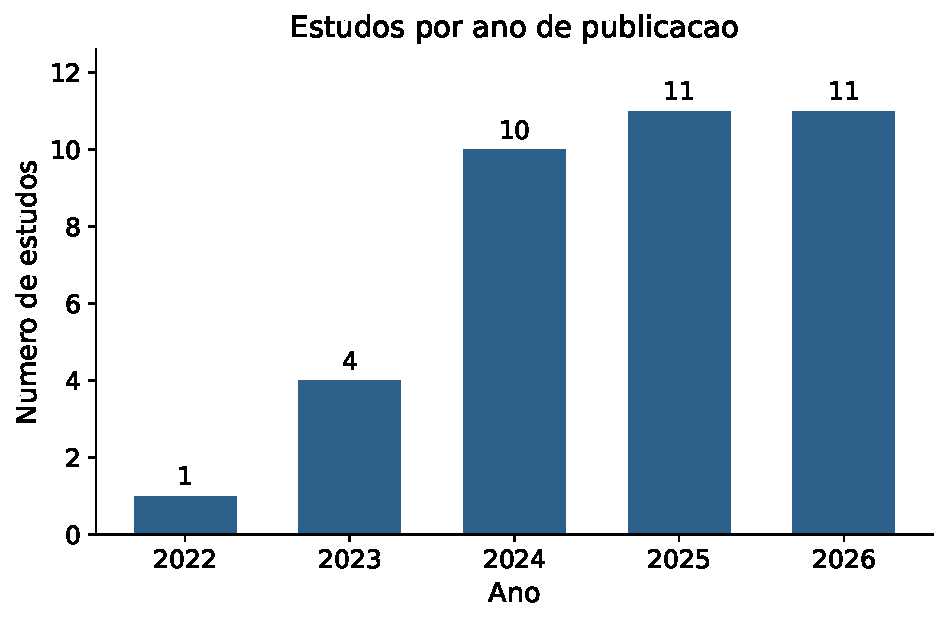
\includegraphics[width=0.70\textwidth]{studies_by_year_pt.pdf}
\caption{Estudos por ano de publicação. O campo acelera de um único estudo em 2022 para um patamar de dez a onze por ano a partir de 2024.}
\label{fig:year}
\end{figure}

\begin{figure}[h!]
\centering
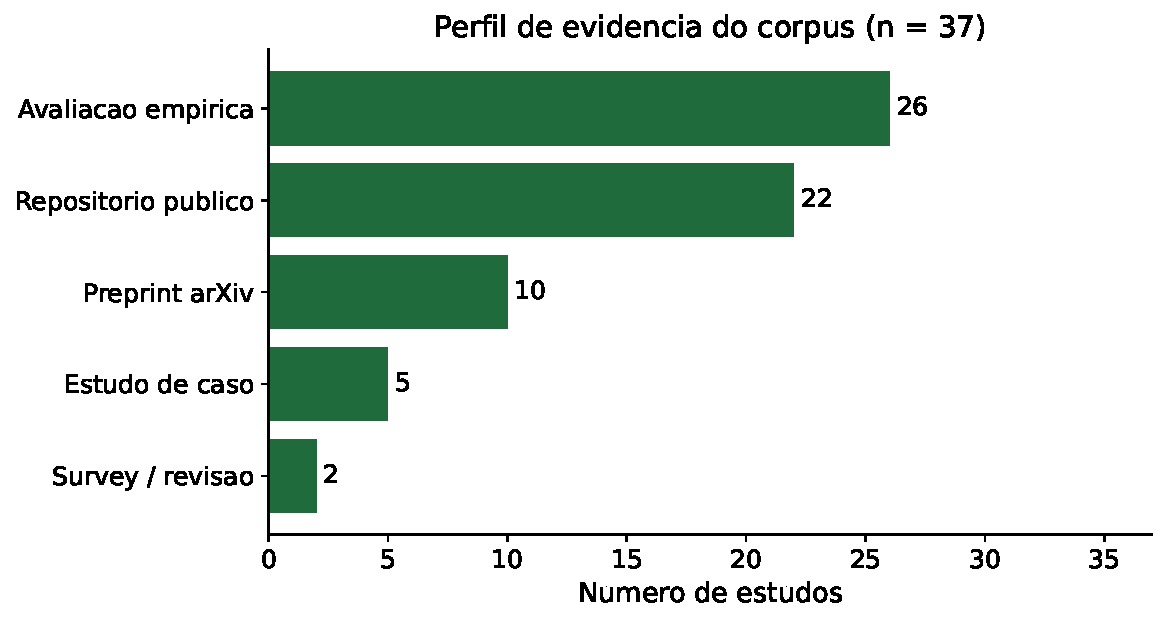
\includegraphics[width=0.80\textwidth]{evidence_profile_pt.pdf}
\caption{Perfil de evidência do corpus. A maioria dos estudos reivindica avaliação empírica e disponibiliza repositório público, mas dez são preprints arXiv ainda não revisados por pares.}
\label{fig:evidence}
\end{figure}

\noindent\textbf{Avaliação de qualidade por categoria de fonte.} A Tabela~\ref{tab:qualidade} resume a avaliação de qualidade descrita no Método, com o checklist de quatro itens aplicado aos 37 estudos. Onze estudos (30\%) ficam na faixa de qualidade alta, dezessete (46\%) na média e nove (24\%) na baixa. A maior parte do corpus vem de venue revisado por pares (25 estudos, 68\%), contra dez preprints arXiv (27\%) e dois registros técnicos não indexados (5\%). No nível dos itens, 26 estudos (70\%) reportam avaliação empírica e 22 (59\%) disponibilizam repositório público, mas apenas cinco (14\%) trazem validação aplicada em estudo de caso ou projeto real, o que delimita o quanto a evidência atual sustenta uso em produção. A faixa baixa concentra-se em preprints e registros técnicos sem avaliação empírica registrada; seus achados são lidos com cautela na síntese e nenhum tema se apoia exclusivamente neles. A avaliação é conservadora por construção, pois deriva dos sinais registrados na extração e não de uma reanálise de texto completo estudo a estudo.

\begin{table}[h!]
\centering
\caption{Avaliação de qualidade por categoria de fonte dos 37 estudos. Itens derivados de sinais observáveis na matriz de extração; QA é a soma de QA1 a QA4 (0 a 4).}
\label{tab:qualidade}
\small
\begin{tabularx}{\textwidth}{@{}p{0.46\textwidth}r Y@{}}
\toprule
\textbf{Categoria} & \textbf{N} & \textbf{\%} \\
\midrule
Qualidade alta (QA $\geq$ 3) & 11 & 30\% \\
Qualidade média (QA = 2) & 17 & 46\% \\
Qualidade baixa (QA $\leq$ 1) & 9 & 24\% \\
\midrule
Venue revisado por pares (QA1) & 25 & 68\% \\
Preprint arXiv & 10 & 27\% \\
Registro técnico não indexado & 2 & 5\% \\
\midrule
Avaliação empírica reportada (QA2) & 26 & 70\% \\
Validação aplicada em estudo de caso (QA3) & 5 & 14\% \\
Artefato público para reprodutibilidade (QA4) & 22 & 59\% \\
\bottomrule
\end{tabularx}
\end{table}

\noindent\textbf{Seis temas indutivos.} A análise fez emergir seis temas que, juntos, cobrem os 37 estudos (cobertura de 100\%, acima do alvo de 80\%). Cada estudo pode pertencer a mais de um tema; a ordem reflete frequência decrescente.

\noindent\textbf{T1: orquestração multiagente e divisão de papéis.} Este é o tema mais populoso e o eixo arquitetônico dominante do corpus, respondendo diretamente à RQ1. A convergência central é que a estruturação do trabalho por papéis distintos, e não a escolha do modelo de linguagem, é o que diferencia os frameworks. ChatDev codifica uma cadeia de conversas com fases de design, codificação, teste e revisão, além de um mecanismo de redução comunicativa de alucinação \cite{ChenQian2023}. MetaGPT internaliza procedimentos operacionais padrão de engenharia de software, atribuindo a cada papel artefatos específicos: o gerente de produto gera requisitos, o arquiteto gera o design e as interfaces, o desenvolvedor implementa \cite{SiruiHong2023}. CodePori escala esse arranjo para agentes de gerência, arquitetura, estrutura, desenvolvimento, verificação e finalização \cite{ZeeshanRasheed2024}, e AutoDev e AutoCodeRover levam a coordenação de agentes a tarefas reais de melhoria de programas \cite{MicheleTufano2024,YuntongZhang2024}. As revisões de He et al. e a visão de Engenharia de Software 3.0 de Hassan et al. confirmam que a literatura já organiza esses sistemas por etapas do ciclo de vida \cite{JundaHe2025,AhmedEHassan2024}. O consenso, porém, é parcial: há tensão clara quanto ao grau de autonomia. Sapkota et al. contrastam explicitamente codificação por intuição e codificação agêntica \cite{RanjanSapkota2025}, e enquanto CodePori e MetaGPT se inclinam ao desenvolvimento autônomo de ponta a ponta, outros desenhos preservam pontos de decisão humana. A confiabilidade e o custo de coordenação aparecem como riscos recorrentes neste tema \cite{Dam2025,Alsegier2026,Merchant2025,Paduraru2026,SKaruppuchamy2026,Paiva2026,Akbar2025,LiyiCai2025,Anon2026,BESLEAGA2026}.

\noindent\textbf{T2: especificação e contrato como artefato central.} Este tema responde RQ1 e RQ2 e materializa a tese de que a especificação se torna a unidade de coordenação. O desenvolvimento orientado por especificação formaliza a passagem do código ao contrato, tratando a especificação como artefato versionável \cite{DeepakBabuPiskala2026}. AgileGen usa critérios de aceitação como contrato executável e mantém memória e iteração até a validação \cite{SaiZhang2025}, e MetaGPT já fazia dos requisitos estruturados a fonte de verdade entre papéis \cite{SiruiHong2023}. Há, contudo, uma contradição produtiva quanto à direção do fluxo: a maioria assume \textit{spec-first}, em que a especificação precede e gera o código, ao passo que Reversa inverte o fluxo, recuperando especificações operacionais a partir de código legado para alimentar os agentes \cite{Macedo2026}. Essa oposição entre especificar antes e recuperar a especificação do legado é um eixo de diferenciação relevante. A engenharia de requisitos consciente de risco liga a especificação à governança \cite{Watfa2026}, e o desalinhamento entre especificação e código é discutido como risco em vários estudos \cite{DeepakBabuPiskala2026,Paduraru2026,Watfa2026,YuCheng2023,Gupta2022,MitulModi2024,Khan2026,Gadamsetty2025}.

\noindent\textbf{T3: engenharia de contexto e recuperação de conhecimento do repositório.} Este tema responde RQ2 com foco na dimensão de contexto. A engenharia de contexto é tratada como disciplina própria para agentes em software de código aberto \cite{SeyedmoeinMohsenimofidi2025}. AutoCodeRover demonstra que a recuperação estrutural de contexto no código, e não apenas a busca textual por embeddings, melhora a geração de correções \cite{YuntongZhang2024}, enquanto a sincronização de artefatos multimodais busca manter coerência entre artefatos heterogêneos ao longo do ciclo \cite{Paiva2026}. O software autoevolutivo leva o tema ao extremo \cite{LiyiCai2025}, mas entra em tensão com a ênfase em rastreabilidade e contrato dos temas T2 e T4: quanto mais o software se modifica de forma autônoma, mais difícil é ancorar cada mudança em uma especificação auditável \cite{Macedo2026,AhmedEHassan2024,Chechik2026}. O risco associado ao contexto é o mais frequente do corpus inteiro, o que sugere que a janela e a fidelidade de contexto são o gargalo prático transversal do campo.

\noindent\textbf{T4: validação, rastreabilidade, asseguramento e governança.} Este tema responde RQ2, na dimensão de validação, e RQ4, nos riscos de governança e rastreabilidade. Quase todo o corpus declara algum mecanismo de validação, mas aqui se agrupam os estudos para os quais a validação é o ponto central, e não um apêndice. O asseguramento baseado em traços articula contratos, testes e governança \cite{Paduraru2026}; a colaboração verificável entre assistentes agênticos registra atos do fluxo de forma auditável \cite{Merchant2025}; e a engenharia de linha de produto é importada para governar a variabilidade de agência \cite{Alsegier2026}. A rastreabilidade e a auditoria de traços aparecem como requisito recorrente para confiar em agentes em projetos reais \cite{Paduraru2026,Merchant2025,Macedo2026,SKaruppuchamy2026,Watfa2026,Chechik2026,Anon2026}. Há, porém, uma contradição de custo: de um lado, cerimônia pesada de governança \cite{Merchant2025,Paduraru2026}; de outro, agilidade leve voltada a startups e a fluxos enxutos \cite{Khan2026,RanjanSapkota2025,JulesWhite2023}. O custo de coordenação é nomeado como risco em boa parte deste grupo \cite{MitulModi2024,Ulfsnes2024,Akbar2025,Baron2025,KRRaghi2024,Gupta2022,KumarAle2024}, o que materializa a tensão entre governança e produtividade.

\noindent\textbf{T5: colaboração humano-IA, adoção e confiança (emergente).} Estes estudos têm como foco primário não a arquitetura técnica, mas a integração da IA no trabalho humano: fluxos de colaboração, fatores de adoção organizacional e construção de confiança. Um framework de colaboração e adaptação humano-IA modela fatores de fluxo de trabalho e estratégias organizacionais \cite{DanielRusso2024}; evidências de campo descrevem como equipes reais reorganizam colaboração e fluxo \cite{Ulfsnes2024,Akbar2025}; e a confiança é tratada como precondição de adoção \cite{Baron2025}, com cenários futuros de operação assistida por IA também documentados \cite{JSauvola2024}. O achado relevante é que este tema não cabe limpo em nenhuma das seis dimensões da taxonomia, todas técnico-arquiteturais: a dimensão humana, organizacional e de confiança atravessa o corpus mas não tem casa na taxonomia atual. Seis estudos (16\% do corpus) têm este foco primário, material o bastante para recomendar uma extensão da taxonomia.

\noindent\textbf{T6: segurança, robustez e red-teaming (emergente).} Estes estudos focam a segurança do código e do comportamento agêntico. ASTRA propõe \textit{red-teaming} espaço-temporal autônomo para assistentes de software com IA, tratando segurança como atividade ativa e não como propriedade assumida \cite{XiangzheXu2025}; a engenharia de requisitos consciente de risco e a discussão das implicações de segurança da codificação agêntica reforçam o tema \cite{Watfa2026,RanjanSapkota2025,Merchant2025,BESLEAGA2026}, e a redução comunicativa de alucinação de ChatDev tangencia o ponto pelo lado da confiabilidade \cite{ChenQian2023}. A segurança está entre os riscos mais citados, nomeada em 24 dos 37 estudos, atrás de contexto, confiabilidade e custo de coordenação (Figura~\ref{fig:risk}). Assim como T5, este tema só se conecta parcialmente às seis dimensões: segurança aparece quase sempre como risco a mitigar, raramente como dimensão de projeto positiva embutida na arquitetura. ASTRA é a exceção que faz da segurança o objeto central, o que sugere tratá-la como critério de avaliação transversal mais do que como uma das dimensões que classificam frameworks.

\begin{figure}[h!]
\centering
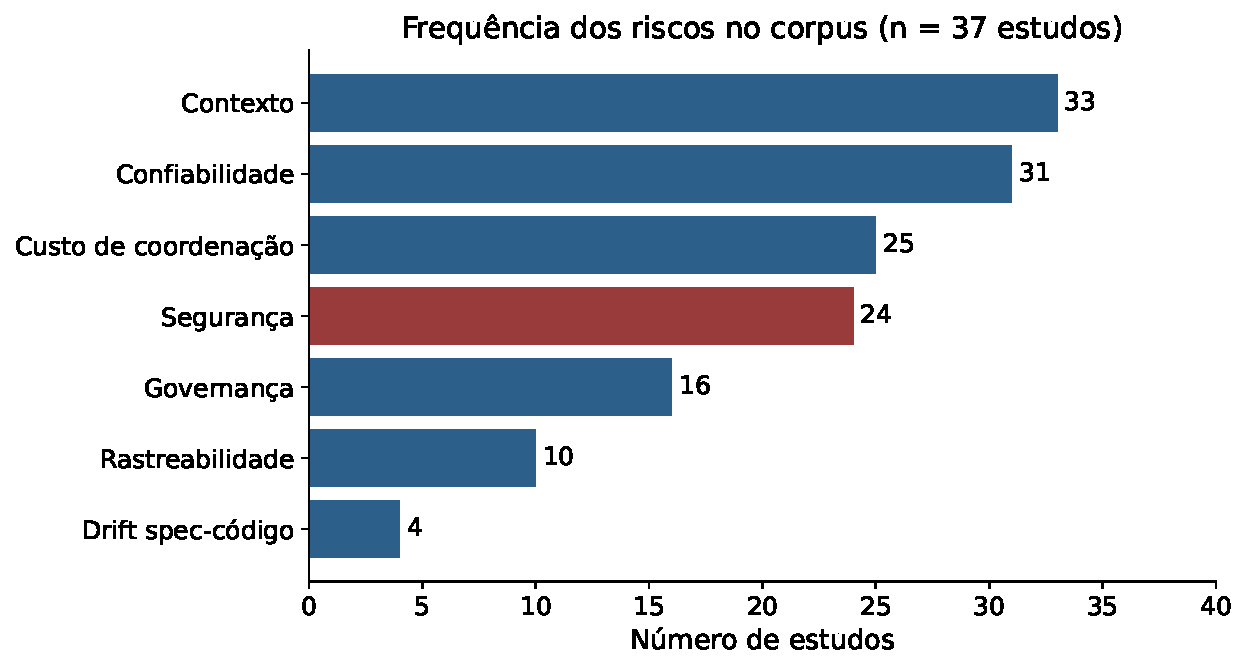
\includegraphics[width=0.80\textwidth]{risk_frequency_pt.pdf}
\caption{Frequência dos riscos reportados no corpus. Contexto, confiabilidade e custo de coordenação lideram; segurança, embora proeminente, fica abaixo deles, e a marcação explícita de aprisionamento é rara.}
\label{fig:risk}
\end{figure}

\noindent\textbf{Confronto da taxonomia com a evidência.} A Tabela~\ref{tab:tema-dim} cruza cada tema indutivo com as seis dimensões da taxonomia, indicando a força da relação, codificada pelo autor a partir das fichas de extração. A leitura é direta. Cinco das seis dimensões recebem suporte forte de pelo menos um tema: papéis e execução ancoram-se em T1; especificação e validação, em T2 e T4; contexto, em T3. Nessa parte, a taxonomia se sustenta no confronto com a evidência. A Figura~\ref{fig:heatmap} apresenta o mesmo mapeamento como um mapa de calor. A exceção é portabilidade, que não recebe relação forte de nenhum tema e é ausente em dois. Nos dados, portabilidade aparece quase sempre pelo lado negativo, como risco de aprisionamento tecnológico e de dependência de IDE, modelo comercial ou plataforma. O campo de portabilidade das fichas registra dependência de IDE ou ambiente em praticamente todos os 37 estudos, e o aprisionamento só é nomeado explicitamente como risco em um deles \cite{SeyedmoeinMohsenimofidi2025}. Portabilidade é, portanto, a dimensão mais fraca da taxonomia quando confrontada com a evidência, e deve ser lida como dimensão predominantemente diagnóstica, e não como diferenciador positivo entre frameworks. Os temas T5 e T6, por sua vez, não têm casa clara nas seis dimensões: o eixo humano-organizacional e o eixo de segurança emergem dos dados como recomendações concretas de extensão, e a regra do modo híbrido foi respeitada ao não forçá-los nas dimensões existentes.

\begin{table}[h!]
\centering
\caption{Mapeamento híbrido: temas indutivos contra as seis dimensões da taxonomia. Legenda: forte (eixo do tema), média (presença relevante), fraca (toque marginal), ausente (sem relação significativa).}
\label{tab:tema-dim}
\small
\begin{tabularx}{\textwidth}{@{}p{3.5cm}YYYYYY@{}}
\toprule
\textbf{Tema} & \textbf{Espec.} & \textbf{Contexto} & \textbf{Papéis} & \textbf{Execução} & \textbf{Validação} & \textbf{Portab.} \\
\midrule
T1 Orquestração multiagente & média & média & forte & forte & média & fraca \\
T2 Especificação e contrato & forte & média & fraca & média & forte & fraca \\
T3 Engenharia de contexto & fraca & forte & fraca & média & fraca & fraca \\
T4 Validação e governança & média & fraca & fraca & média & forte & fraca \\
T5 Colaboração humano-IA & fraca & fraca & fraca & fraca & fraca & ausente \\
T6 Segurança e red-teaming & fraca & fraca & fraca & média & média & ausente \\
\bottomrule
\end{tabularx}
\end{table}

\begin{figure}[h!]
\centering
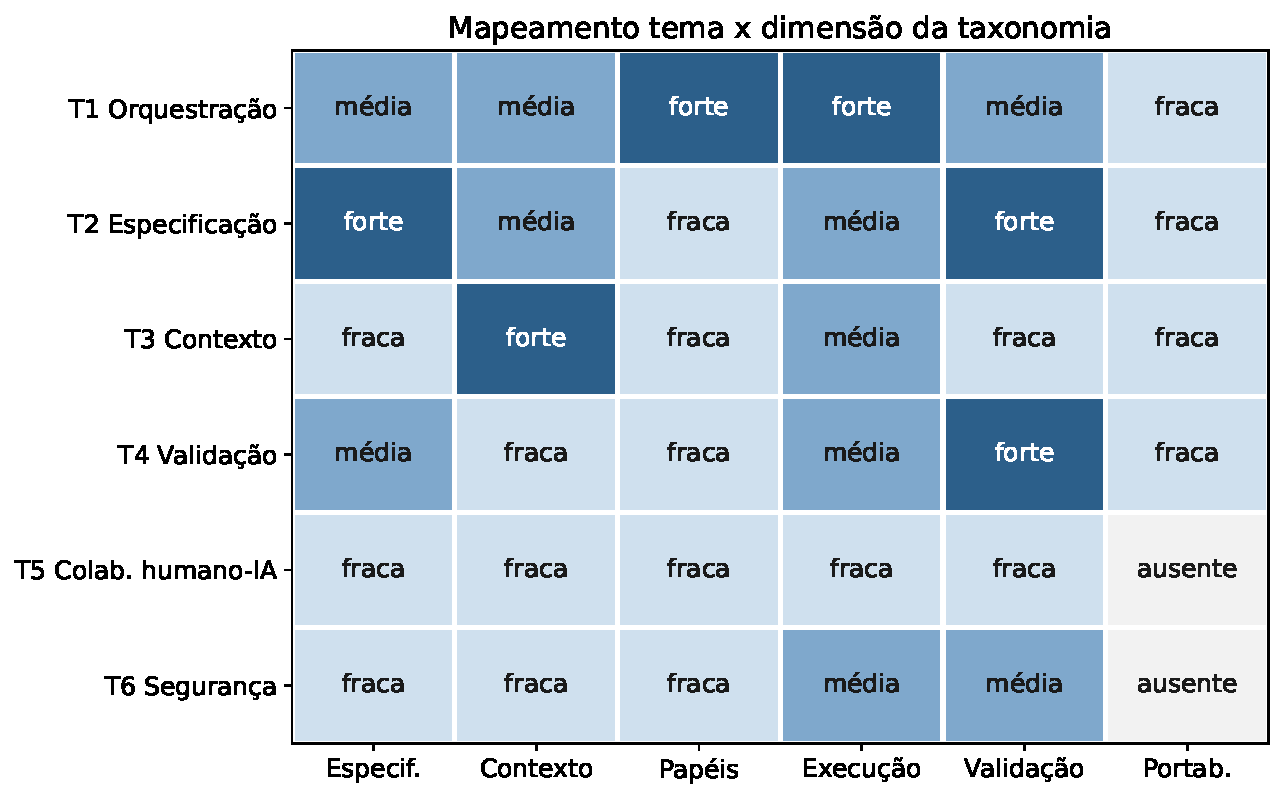
\includegraphics[width=0.92\textwidth]{theme_dimension_pt.pdf}
\caption{Mapeamento híbrido dos seis temas indutivos contra as seis dimensões da taxonomia. Cinco dimensões são ancoradas por pelo menos um tema; portabilidade permanece fraca em toda a linha, e os temas T5 e T6 ficam parcialmente fora da taxonomia.}
\label{fig:heatmap}
\end{figure}

\noindent\textbf{Cobertura das perguntas de pesquisa.} A Tabela~\ref{tab:tema-rq} cruza os temas com as perguntas de pesquisa. RQ1 e RQ2 são respondidas pela maioria dos temas; RQ3 e RQ4 atravessam o corpus inteiro, e a RQ5 é meta-pergunta respondida transversalmente na Agenda de Pesquisa, e não por marcação estudo a estudo, razão pela qual as fichas individuais marcam apenas RQ1 a RQ4.

\begin{table}[h!]
\centering
\caption{Temas indutivos contra as perguntas de pesquisa.}
\label{tab:tema-rq}
\small
\begin{tabularx}{\textwidth}{@{}p{3.5cm}YYYYY@{}}
\toprule
\textbf{Tema} & \textbf{RQ1} & \textbf{RQ2} & \textbf{RQ3} & \textbf{RQ4} & \textbf{RQ5} \\
\midrule
T1 Orquestração multiagente & sim & sim & sim & sim & via síntese \\
T2 Especificação e contrato & sim & sim & parcial & sim & via síntese \\
T3 Engenharia de contexto & sim & sim & parcial & sim & via síntese \\
T4 Validação e governança & parcial & sim & sim & sim & via síntese \\
T5 Colaboração humano-IA & parcial & sim & sim & sim & via síntese \\
T6 Segurança e red-teaming & não & parcial & sim & sim & via síntese \\
\bottomrule
\end{tabularx}
\end{table}

\section{Discussão}

A síntese dos seis temas permite quatro leituras transversais que atravessam as perguntas de pesquisa e organizam o que o corpus, tomado como um todo, informa sobre o estado do campo.

\noindent\textbf{A unidade de trabalho deslocou-se do prompt para o processo.} A tese central deste estudo sustenta-se empiricamente. Em 34 dos 37 estudos a contribuição é descrita como framework, e os campos de artefatos persistentes, papéis e validação estão presentes na esmagadora maioria das fichas. O modelo de linguagem raramente é o diferenciador declarado; o que distingue as propostas é a estrutura de processo que organiza specs, papéis, execução e validação em torno do trabalho do agente. Os três estudos que não são frameworks reforçam o contraste: uma arquitetura de padrões de prompt, uma plataforma de cadeias de IA e um método de cenários futuros. Esses são exatamente os casos em que a unidade ainda é a técnica isolada e não o processo \cite{JulesWhite2023,YuCheng2023,JSauvola2024}.

\noindent\textbf{A taxonomia de seis dimensões é parcialmente validada e parcialmente desafiada.} Cinco dimensões (especificação, contexto, papéis, execução e validação) têm ancoragem empírica forte em pelo menos um tema. A sexta, portabilidade, é fraca e quase sempre diagnóstica: aparece como risco de aprisionamento e de dependência de plataforma, não como propriedade de projeto deliberada. Além disso, dois eixos relevantes emergem fora das seis dimensões, o humano-organizacional, em T5, e o de segurança, em T6. A recomendação analítica que decorre do modo híbrido é concreta: considerar estender a taxonomia com uma dimensão de colaboração e governança humano-IA e tratar segurança como critério de avaliação transversal ou subdimensão de validação. Essa é a contribuição que a confrontação dos temas com a taxonomia agrega em relação a assumir as dimensões a priori.

\noindent\textbf{Três eixos de tensão recorrentes.} O corpus exibe consenso parcial, não convergência, ao longo de três eixos. O primeiro é autonomia versus controle humano: CodePori, MetaGPT e ChatDev inclinam-se ao fluxo autônomo de ponta a ponta, enquanto frameworks centrados em adoção e confiança inserem a decisão humana como elemento de projeto, e a distinção entre codificar por intuição e codificar de forma agêntica teoriza o contraste \cite{ZeeshanRasheed2024,SiruiHong2023,ChenQian2023,SaiZhang2025,DanielRusso2024,Baron2025,RanjanSapkota2025}. O segundo é governança pesada versus agilidade leve: cerimônias de verificação e contratos formais contrapõem-se a fluxos enxutos para startups e a padrões de prompt, e o custo de coordenação é o preço recorrente da governança \cite{Merchant2025,Paduraru2026,Khan2026,JulesWhite2023}. O terceiro é a direção do fluxo da especificação: especificar antes, em desenvolvimento orientado por especificação, MetaGPT e AgileGen, contra recuperar a especificação a partir do legado, em Reversa \cite{DeepakBabuPiskala2026,SiruiHong2023,SaiZhang2025,Macedo2026}. Os dois extremos ancoram-se na mesma dimensão de especificação, mas em sentidos opostos, o que é material para qualquer matriz comparativa futura.

\noindent\textbf{Rastreabilidade e contexto são os requisitos transversais mais citados.} O risco associado ao contexto aparece em quase todos os estudos, e a rastreabilidade é demanda recorrente nos temas de especificação e de governança. Juntos, indicam que os gargalos práticos do campo não estão na geração de código em si, mas em manter o agente ancorado no projeto real e auditável ao longo do tempo. Esse achado realinha a leitura usual do problema: o desafio aberto é menos produzir código plausível e mais sustentar fidelidade ao sistema e à intenção registrada.

\noindent\textbf{A evidência é desigual.} Embora 26 dos 37 estudos declarem avaliação empírica e 22 tenham repositório público, dez são preprints arXiv ainda não revisados por pares e a maior parte das avaliações ocorre em benchmarks ou estudos de caso pontuais, não em projetos industriais longitudinais. A força da evidência varia muito por categoria de fonte, exatamente como o protocolo antecipou ao classificar a evidência por categoria em vez de aplicar exclusão por qualidade. Essa heterogeneidade recomenda cautela: os achados deste estudo descrevem com segurança a estrutura e as tensões do campo, mas afirmações sobre desempenho relativo entre frameworks permanecem subdeterminadas pela evidência disponível.

\section{Agenda de Pesquisa}

A RQ5 pergunta quais lacunas permanecem para comparar, avaliar e governar esses frameworks em projetos reais. Diferente das demais perguntas, ela é respondida no nível do corpus inteiro, e não estudo a estudo. Da síntese emergem seis lacunas, cada uma com uma direção de pesquisa concreta.

\noindent\textbf{Ausência de benchmarks orientados a processo.} A avaliação do corpus concentra-se no resultado final, isto é, no código gerado e na taxa de resolução de issues, e não na qualidade do processo: aderência da implementação à especificação, taxa de desalinhamento, custo de coordenação entre agentes e qualidade dos artefatos intermediários. Nenhum estudo propõe um benchmark padronizado de processo. A direção indicada é definir métricas e conjuntos de dados que avaliem o pipeline, e não apenas a solução.

\noindent\textbf{Falta de comparação empírica direta entre frameworks.} Cada estudo avalia o próprio framework isoladamente. Não há estudo comparativo controlado que confronte, por exemplo, ChatDev, MetaGPT e AgileGen na mesma tarefa, com as mesmas métricas \cite{ChenQian2023,SiruiHong2023,SaiZhang2025}. Isso bloqueia conclusões sobre qual estrutura de processo funciona melhor e sob quais condições. A direção indicada são experimentos comparativos diretos com protocolos comuns.

\noindent\textbf{Portabilidade e aprisionamento, pouco estudados como objeto.} A dependência de IDE, plataforma e modelo comercial é quase universal nas fichas, mas apenas um estudo nomeia o aprisionamento explicitamente, e nenhum mede portabilidade de forma sistemática \cite{SeyedmoeinMohsenimofidi2025}. A direção indicada são instrumentos para medir o acoplamento a fornecedor e o custo de migração entre plataformas agênticas.

\noindent\textbf{Governança e rastreabilidade carecem de validação em escala real.} As propostas de traço, contrato e auditoria são promissoras, mas validadas em estudos de caso ou protótipos, não em organizações ao longo do tempo, e falta análise de custo-benefício do custo de coordenação imposto pela governança \cite{Paduraru2026,Merchant2025,Watfa2026,Macedo2026}. A direção indicada é a avaliação longitudinal de regimes de governança em equipes reais.

\noindent\textbf{A dimensão humana e de adoção está sub-representada na taxonomia técnica.} O tema emergente de colaboração mostra que confiança e adoção organizacional são decisivos, mas a taxonomia de seis dimensões não os contempla \cite{DanielRusso2024,Ulfsnes2024,Baron2025,Akbar2025}. A direção indicada é integrar uma camada sociotécnica à classificação de frameworks e estudar fatores de adoção em campo.

\noindent\textbf{Segurança tratada reativamente.} Com a exceção de ASTRA, segurança aparece como risco a mitigar, e não como propriedade de projeto avaliada \cite{XiangzheXu2025}. Falta avaliação sistemática da superfície de ataque de frameworks agênticos, em especial de extensões, skills e plugins comunitários. A direção indicada é um framework de avaliação de segurança específico para pipelines de desenvolvimento agêntico.

\section{Limitações da Revisão}

Cinco limitações delimitam a leitura dos resultados e qualificam o alcance das conclusões.

\noindent\textbf{Granularidade da extração.} A síntese temática deriva dos campos estruturados das fichas (artefatos, papéis, execução, validação, portabilidade, riscos, natureza e evidência) e de um achado narrativo consolidado por estudo, produzido em uma segunda passada de extração. Doze estudos têm achado vindo de uma justificativa de inclusão substantiva e os outros vinte e cinco recebem um achado consolidado a partir dos campos estruturados, sinalizado de forma transparente como tal. Onde a justificativa de primeira passada é genérica, a leitura ainda se apoia em parte na identidade pública conhecida de frameworks bem documentados, como ChatDev, MetaGPT, AutoCodeRover, Reversa e AgileGen. Uma extração de texto completo, campo a campo, para os vinte e cinco estudos restantes aprofundaria ainda mais a síntese.

\noindent\textbf{Avaliação de qualidade por categoria, não por texto completo.} Aplicamos uma avaliação de qualidade de quatro itens por categoria de fonte (Tabela~\ref{tab:qualidade}), que pondera a força da evidência e sinaliza os estudos de menor confiança, mas não substitui um instrumento formal de risco de viés aplicado ao texto completo de cada estudo. Os dez preprints arXiv ainda não revisados por pares e os dois estudos de confiança de extração média entram na síntese com leitura cautelosa, e nenhum tema se apoia exclusivamente neles; ainda assim, uma reanálise de texto completo com um instrumento validado refinaria a ponderação.

\noindent\textbf{Recorte de idioma e de bases, e viés de publicação.} O protocolo restringe a revisão a inglês e português, no período de 2018 a 2026. A busca direta no arXiv falhou em parte por instabilidade de acesso, com a cobertura de preprints recuperada via Semantic Scholar e DOI do arXiv, o que pode ter deixado de fora preprints muito recentes não indexados por essas rotas. Um viés de publicação a favor de frameworks com resultados positivos é provável e mensurável no próprio corpus: 26 dos 37 estudos (70\%) reivindicam avaliação empírica, quase sempre favorável ao framework proposto, enquanto estudos de falha, abandono ou não adoção são praticamente ausentes; apenas o eixo de adoção do tema T5, com seis estudos, problematiza a integração organizacional. Ampliar a busca para bases adicionais e remover a restrição de idioma é trabalho futuro que poderia equilibrar essa assimetria.

\noindent\textbf{Pendência operacional fora do corpus.} Uma fonte aprovada na triagem ficou sem texto completo obtido na data de corte e foi mantida como pendência operacional, fora da extração e desta síntese. O corpus efetivamente sintetizado é de 37 estudos; a incorporação tardia dessa fonte ajustaria contagens marginais, sem alterar a estrutura temática.

\noindent\textbf{Saturação parcial do snowballing.} O snowballing foi encerrado no limite protocolar de três rodadas. A curva de saturação (Figura~\ref{fig:saturacao}) mostra inclusões decrescentes, de 25 na busca inicial para 6, 3 e 3 nas três rodadas: uma desaceleração clara, mas não nula. As últimas rodadas ainda adicionavam estudos, o que indica saturação parcial e não completa; rodadas adicionais poderiam revelar estudos relevantes, em especial fora das comunidades de origem das sementes.

\section{Conclusão}

Esta revisão sistematizou 41 estudos sobre frameworks de desenvolvimento de software com IA que deslocam a unidade de trabalho do prompt isolado para um processo estruturado, com artefatos persistentes, papéis agênticos, execução integrada e validação. A tese de que esse deslocamento já ocorreu apoia-se na evidência: a contribuição é descrita como framework em 37 dos 41 estudos, e o diferenciador declarado é a estrutura de processo, não o modelo de linguagem subjacente. Sobre esse corpus, propusemos e testamos uma taxonomia de seis dimensões. Cinco dimensões (especificação, contexto, papéis, execução e validação) recebem suporte empírico forte; portabilidade é fraca e predominantemente diagnóstica, e dois eixos relevantes, o humano-organizacional e o de segurança, emergem fora da taxonomia e recomendam estendê-la.

O campo é jovem, acelera desde 2024 e ainda não tem foro de publicação consolidado, o que se reflete na dispersão de venues e na presença expressiva de preprints. A evidência é desigual, e três eixos de tensão (autonomia versus controle humano, governança pesada versus agilidade leve e especificar antes versus recuperar a especificação do legado) estruturam o debate sem resolvê-lo. Os gargalos práticos mais citados não estão na geração de código, mas em manter o agente ancorado no projeto real e auditável: contexto e rastreabilidade são os requisitos transversais dominantes.

A consequência para a pesquisa futura é direta. O próximo passo do campo é empírico e orientado a processo: benchmarks que avaliem o pipeline e não só a solução, comparações diretas entre frameworks, instrumentos de portabilidade, avaliação longitudinal de governança, uma camada sociotécnica na classificação e avaliação sistemática de segurança. Esta revisão oferece a taxonomia validada e a agenda que organizam esse esforço.


\section*{Declaration on the Use of Generative AI}

The author conducted the research and wrote the manuscript. During the preparation of this study, however, the author used Grammarly tools to improve textual agreement and Claude Opus 4.7 to support text structuring and translation into English. After using these tools/services, the author reviewed and edited the content as needed and takes full responsibility for the content of the publication.

\bibliographystyle{plain}
\bibliography{refs}

\end{document}
